%Plantilla anteproyecto TFG
%Última modificación: 28 de mayo de 2021
\documentclass[12pt,oneside,a4paper]{article}
\usepackage[spanish]{babel}
\usepackage[utf8]{inputenc}
\usepackage{graphicx}
\usepackage{amsmath}
\usepackage{amssymb}
\usepackage{xcolor}
\usepackage{subfigure}
\usepackage{url}
\usepackage{float}
\linespread{1}
\usepackage{multirow}
\usepackage{colortbl}
\usepackage{rotating}
\usepackage[pagebackref=true,breaklinks=true,letterpaper=true,colorlinks=true,linkcolor=black,bookmarks=true]{hyperref}
\usepackage{setspace}

\usepackage[spanish]{babel}
\usepackage[utf8]{inputenc}

\usepackage{transparent}
\usepackage{eso-pic}
 
\usepackage{blindtext}

\makeindex
\setlength{\parskip}{1\baselineskip}
\parindent 1cm
\sloppy


%Opciones que debes descomentar mientras estemos revisando el anteproyecto
\usepackage{lineno}
\linenumbers


\usepackage[pagebackref=true,breaklinks=true,letterpaper=true,colorlinks,bookmarks=true]{hyperref}


%lista de palabras que Latex no parte bien
\hyphenation{pa-la-bras lis-ta}

\begin{document}
\AddToShipoutPicture{
\put(0,0){
\parbox[b][\paperheight]{\paperwidth}{%
\vfill
\centering
{\transparent{0.05}
\includegraphics[scale=1.5]{figuras/logo-uah.jpg}}%
\vfill
}
}
}

\thispagestyle{empty}

\begin{center}

\begin{large}
UNIVERSIDAD DE ALCALÁ\\
Escuela Politécnica Superior\\
\end{large}
\vspace{4cm}


\begin{spacing}{2} % Ajusta el factor según tus necesidades
\begin{Huge}\textbf{\textit{Innovación Tecnológica en la Evaluación Geriátrica: Automatización de Pruebas SPPB mediante Aplicación Móvil y Plataforma Web}}\end{Huge}
\end{spacing}



\vspace{1cm}


\textbf{ANTEPROYECTO FIN DE GRADO}

\vfill
\hline
Abril - 2024

\end{center}

\begin{flushright}
\textit{Autor - \textbf{F. Javier Redondo García}} \\
\textit{Tutor - \textbf{Sergio Caro Álvaro}} \\
\textit{Cotutora - \textbf{Ana Jiménez Martín}}

\end{flushright}




\newpage
\section{Introducción}
\hline

Actualmente, con la esperanza de vida tan alta, el envejecimiento de la población supone un problema y un reto para muchas especialidades, que buscan que las personas tengan un envejecimiento saludable, retrasando la fragilidad.

 Se pretende, entre otras cosas, detectar el decaimiento físico en sus etapas más tempranas para intentar retrasar el estado de fragilidad. Para ello se utiliza el Test de evaluación del desempeño físico \cite{welch2021short} (SPPB) del adulto mayor como ayuda a la valoración geriátrica integral. \\
El Test consiste en la realización de tres pruebas a cada uno de los pacientes. El protocolo de las pruebas es el siguiente: \\
\begin{itemize}
\item Prueba de equilibrio: Se debe aguantar 10 segundos en tres posiciones diferentes (pies juntos, semitándem y tándem), sin ningún tipo de apoyo. \\
\item Prueba de velocidad de la marcha en 4 metros: Se mide el tiempo que tarda el paciente en recorrer 4 metros en línea recta. Se realizan dos pruebas.\\
\item Prueba de levantarse de la silla 5 veces: El paciente debe levantarse de la silla lo más rápido que pueda sin utilizar los brazos. Se mide el tiempo que tarda en hacerlo.
\end{itemize}
Según el desempeño que el paciente haya tenido en las pruebas, se le asignan unos puntos, que son utilizados por el personal sanitario como una herramienta de ayuda a la detección de fragilidad.

Para la realización de este proyecto, se cuenta con el apoyo del grupo de investigación GEINTRA, que proporciona tres dispositivos, uno para cada una de las pruebas SPPB, que transmiten datos sin procesar a traves de tecnología Bluethooth.





\section{Objetivo}
\hline
El objetivo principal del proyecto es facilitar, agilizar y mejorar la intervención médica con ayuda tecnológica, creando un sistema que automatice las pruebas SPPB de tal manera que puedan realizarse en atención primaria, descongestionando así cansultas de geriatría. 
Para llegar a este objetivo, el proyecto se divide en objetivos parciales. Estos objetivos parciales son, en primer lugar, la elección del gestor de bases de datos adecuado, en segundo lugar, el desarrollo de una aplicación móvil, y por último, el desarrollo de una página web.

Con respecto al gestor de la base de datos, actualmente, existen diferentes tipos de bases de datos atendiendo a su estructura y al modelo de datos que utilizan, siendo este un elemento fundamental para proyectos de este estilo. Es fundamental conocer bien los datos que se utilizan y almacenarlos de una manera óptima y accesible para los sistemas externbos. En este apartado se deberá hacer un análisis de qué tipos de datos vamos a tener y qué estructura es óptima para almacenarlos, eligiendo así el gestor más adecuado para el trabajo.

En cuanto a la aplicación móvil, hoy en día está sumamente extendido el uso de Smartphones que tienen conexión a internet, Bluethooth y un alcance de procesamiento muy potente. Sabiendo esto, se pretende desarrollar una aplicación que, conectada con los dispositivos proporcionados por GEINTRA, recoja los datos en crudo y haga todo el procesamiento, convirtiendo los datos en crudo en información útil para el personal sanitario. Desde esta aplicación el facultativo podrá dar de alta al paciente y realizarle las pruebas, con una interfaz sencilla y guiada hasta que las pruebas se hayan terminado y decida si subirla a la base de datos, quedando de esta forma guardada la prueba y accesible para su visualización en la página web. Este dispositivo deberá estar conectado a internet para, una vez terminada la prueba, subir la información a la base de datos, donde quedará registrada y estructurada.

Por último, se pretende visualizar la información en un punto diferente a donde se recogen los datos. Para esto se desarrolla una web donde el personal sanitario pueda visualizar la información de cada paciente, ver las pruebas que ha realizado y poder consultar un histórico. Esta web contiene información sensible de cada paciente, por lo que se debe trabajar en un proceso de autenticación con una seguridad fiable. Se debe poder gestionar un rol para las personas que accedan a la web, y dando la capacidad de visualizar la información solo a ciertos usuarios. Para esta gestión, se establecerá un rol de administrador, que tendrá la capacidad de dar permisos o quitarlos a las cuentas de usuario que se registren en la web. Al registrarse por primera vez, el usuario no podrá ver nada hasta que el administrador le habilite.

Estos tres sistemas deben estar conectados y actualizarse automáticamente cuando haya algún cambio en cualquiera de ellos. Se pretende que sea una interfaz sencilla e intuitiva

\begin{figure}[H]
  \centering
  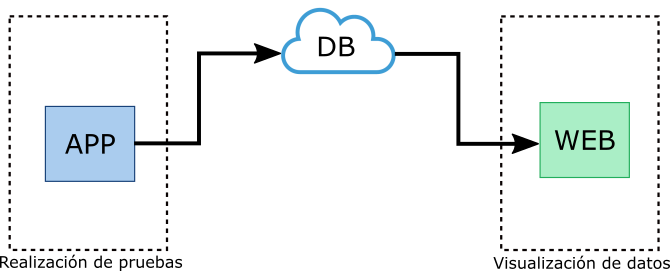
\includegraphics[width=15cm]{anteproyecto/figuras/tfg_diagramabloques_simple.png}
  \caption{Diagrama de bloques del funcionamiento básico del proyecto}
  \label{fig:ejemplo}
\end{figure}


\section{Metodología y plan de trabajo}\index{Metodología} \\
\hline
La propuesta se compone de cinco tareas fundamentales, que se enumeran a continuación: 

\begin{enumerate}


\item    Base de datos \\
\begin{enumerate}
    I.   Seleccion de los tipos de datos a utilizar \\
    II. Decidir la estructura óptima\\
    III. Elección y preparación del gestor de bases de datos adecuado\\
\end{enumerate}
   
\item  Aplicacion movil\\
\begin{enumerate}
    I. Instalación y preparación del entorno de programación\\
    II. Definir el esquema de la APP con ayuda de diagramas\\
    III. Desarrollo del backend\\
    IV. Desarrollo del frontend\\
\end{enumerate}

\item  Servidor web\\
\begin{enumerate}
    I. Intalación y preparación del entorno de programación\\
    II. Definir el esquema de la web con ayuda de diagramas\\
    III. Desarrollo de autenticación y permisos\\
    IV. Desarrollo de la interfaz de usuario\\
\end{enumerate}

\item Comprobación de funcionamiento\\
\begin{enumerate}
    I. Interconexión entre base de datos, APP y web\\
    II. Realización de pruebas\\
\end{enumerate}

\item    Redacción de la memoria \\
\end{enumerate}  \\





\newpage

\section{Cronograma de actividades}
\hline

La planificación temporal correspondiente a estas fases está definida del siguiente modo: 
\begin{table}[H]
\begin{tabular}{|l|c|c|}
\hline
 \cellcolor[HTML]{DAE8FC}Nombre de la tarea& \multicolumn{1}{|l|}{\cellcolor[HTML]{DAE8FC}Código} & \multicolumn{1}{|l|}{\cellcolor[HTML]{DAE8FC}Duración (meses)}   \\ \hline
 Elección y organización de los datos a utilizar& T1&                                                   0.5\\ \hline
                              Desarrollo de aplicación para Smartphone& T2&                                                   1.5\\ \hline   Desarrollo Web& T3& 1.5\\ \hline   Comprobación de funcionamiento&                                                    T4& 2.5\\ \hline
                              Redacción de la memoria                           &                                                    T5& 3.5\\ \hline
\end{tabular}
\caption{Planificación temporal}
\end{table}

\begin{figure}[H]
  \centering
  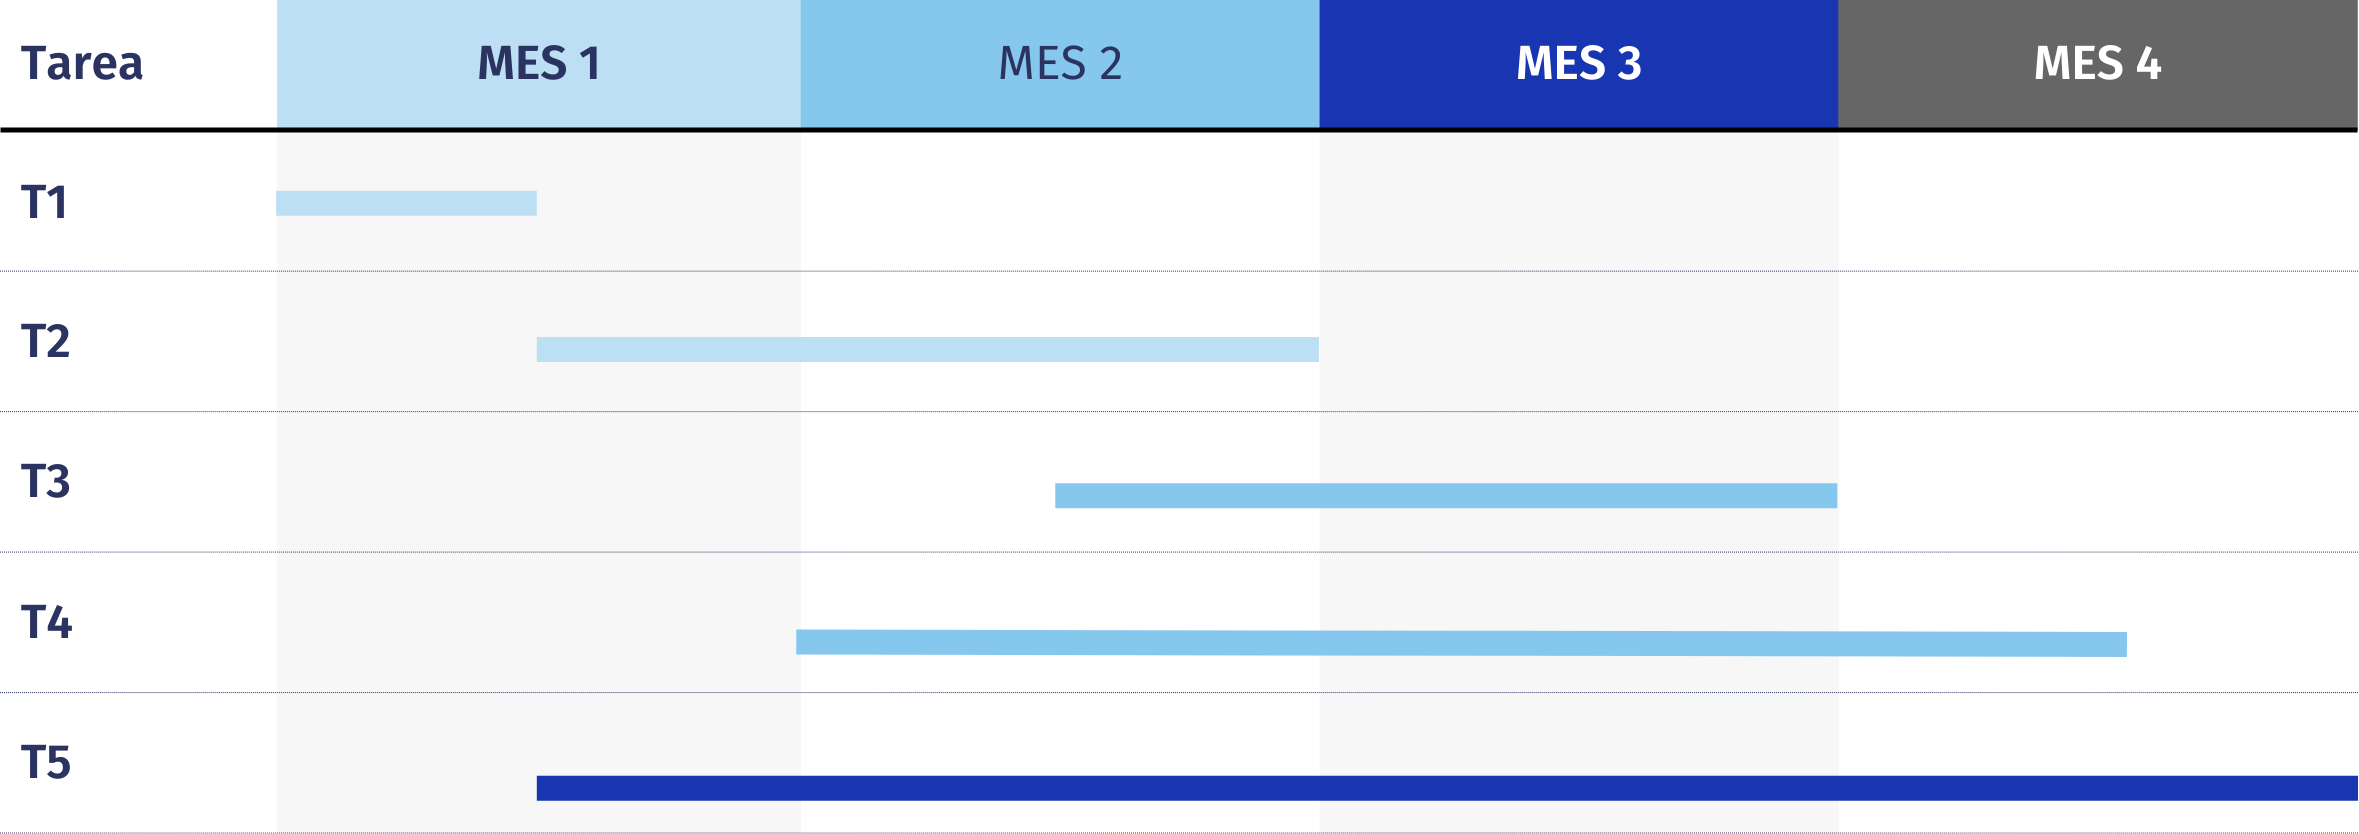
\includegraphics[width=15cm]{anteproyecto/figuras/TareaS_GANTT.png}
  \caption{Diagrama de Gantt}
  \label{fig:ejemplo}
\end{figure}


\section{Medios}
\hline

\textbf{A. Medios Hardware requeridos}
\begin{itemize}
    
    \begin{itemize}
        \item \textbf{Plataforma de equilibrio*} \\
        Esta plataforma se coloca en el suelo y tiene el dibujo de cómo el paciente debe estar colocado al hacer la prueba de equilibrio, según marca el estándar de las pruebas SPPB (paralelo, semi-tándem y tándem). Tiene LEDs que se iluminan cuando se hace presión sobre cada una de las posiciones. Tiene un sistema BlueThooth para conectar con el dispositivo móvil y mandarle los datos en crudo.
        \item \textbf{IMU*} \\
        Destinada a colocarse en el muslo del paciente, manda por BlueThooth datos en crudo de la posición de este en el espacio
        \item \textbf{Sensor ToF* (Time-of-Flight, Tiempo de Vuelo en español)}
        Colocado sobre un trípode, este sensor manda vía BlueThooth datos de la distancia en tiempo real del objeto más cercano al sensor. En el caso del proyecto será el paciente realizando la prueba de velocidad de la marcha
        \item \textbf{Smatphone} \\
        Se hará uso de un teléfono móvil con sistema operativo Android versión 11 o superior. Este teléfono debe tener acceso a internet para poder comunicarse con la base de datos. \\
        \item \textbf{Ordenador personal (PC)} \\
        Que tenga instalado el sistema operativo Windows y un mínimo de 8Gb de memoria RAM
    \end{itemize}
    
\textit{*Dispositivos proporcionados por el grupo de investigación GEINTRA} \\
\\

\textbf{B. Medios Software requeridos}

    \begin{itemize}
        \item \textbf{Android Studio} \\
        Se utilizará para todo el desarrollo de la aplicación móvil y usará mínimo la versión 27 de SDK  \cite{hohensee2014introduccion}. \\
        \item \textbf{Visual Studio Code} \\
        Editor de código fuente que se utilizará para todo el desarrollo de la Web \\
        \item \textbf{Angular} \\
        Framework de desarrollo frontend que ofrece un conjunto de herramientas completo y potente, que puede ser ideal para el objetivo del proyecto \cite{wilken2018angular}. Se utilizará con el lenguaje de programación Typescript, que trabaja sobre JavaScript y que permite añadir características estáticas de tipo, clases y módulos opcionales a JS. \\
        \item \textbf{Gestor de base de datos} \\
Pendiente de elección \\
        \item \textbf{GitHub} \\
        Como herramienta de control de versiones \\
        \item \textbf{Overleaf} \\
        Plataforma online para la edición y compilación de documentos escritos en el sistema de composición de textos \LaTeX \cite{wikibook}\\
    \end{itemize}
    
\end{itemize}









%Bibliografía


\bibliography{bibliografia-tfc}
\bibliographystyle{ieeetr}


\end{document}
